\documentclass{article}

\usepackage[printqrbox=false,printhint=false,printanswer=true,printmarkingguide=false,printdraftpaper=false]{unswalgos}

\usepackage{tikz}
\usetikzlibrary{patterns}
\usetikzlibrary{shapes,fit}
\usepackage{tkz-fct}
\usepackage{wrapfig}
\usepackage{subfig}

\usepackage{mathtools}
\usepackage{amssymb}
\usepackage{booktabs,multicol,multirow}
\usepackage{wasysym}
\usepackage{tcolorbox}

\DeclareMathOperator*{\argmax}{arg\,max}
\DeclareMathOperator*{\argmin}{arg\,min}
\DeclareMathOperator{\NAND}{NAND}
\DeclareMathOperator{\AND}{AND}
\DeclareMathOperator{\OR}{OR}
\DeclareMathOperator{\NOT}{NOT}

\usepackage{xspace}

\fancyfoot[L]{\leftmark}
\fancyfoot[R]{\rightmark}

\usepackage{graphicx}
\usepackage{float}
\usepackage{subfigure}

\usepackage{framed}
% This enables new paragraphs without indentation
\usepackage[parfill]{parskip}

\newcommand{\sem}{22T2}
\newcommand{\semester}{Term 2, 2022}
\SubjectNo{COMP3151}
\newcommand{\taskname}{Homework 7}
\Institution{Jinghan Wang, z5286124} % Replace this with your name and zID


\begin{document}

\setcounter{question}{0}

\begin{Question} [\large\textbf {Process algebra{[5 points]}}]
    We saw a large number of algebraic laws of CCS this Wednesday. Here are some more proposed laws. Briefly discuss the merits of each proposed law, and whether you think it should be accepted. If you think it should be accepted, give an informal intution for why; if you think not, give a concrete example where it has absurd consequences.

\begin{Subquestion}
    $P\ |\ P = P$
    
\begin{answer}
    Answer:
    \begin{quote}
        I think so. $|$ means parallel. Suppose $Clock = P\ |\ P$, $Clock = P.P + P.P + P$, This is true when the starting point and the key point are the same, that is, $P$ is self-cycling.\\
    \end{quote}
\end{answer}
\end{Subquestion}


\begin{Subquestion}
    $P\ \backslash\  b\ \backslash\ b = P\ \backslash\ b$
    
\begin{answer}
    Answer:
    \begin{quote}
        I think so, because $ P\ \backslash\  b$ means the action $b$ and  $\overline{b} $may not be executes in $P$,  $ P\ \backslash\  b\ \backslash\ b$ means the action $b$ and  $\overline{b} $may not be executes in $P\ \backslash\  b$, both of them have same meanings.\\
    \end{quote}
\end{answer}
\end{Subquestion}


\begin{Subquestion}
    $(a.P)\ |\ (a.Q)=a.(P\ |\ Q)$
    
\begin{answer}
    Answer:
    \begin{quote}
        I think it is not. Because, $a.(P\ |\ Q)$ means that process $a$ must finish before process $P$ or $Q$, but $(a.P)\ |\ (a.Q)$ can existed that $a.P.a.Q$, which process $a$ do after $P$ or $Q$.\\
    \end{quote}
\end{answer}
\end{Subquestion}
\end{Question}


\clearpage
\setcounter{question}{1}

\begin{Question} [\large\textbf {Ricart-Agrawala Algorithm{[4 points]}}]
    Pseudocode of the Ricart-Agrawala Algorithm is:
\begin{figure}[H]
    \centering 
    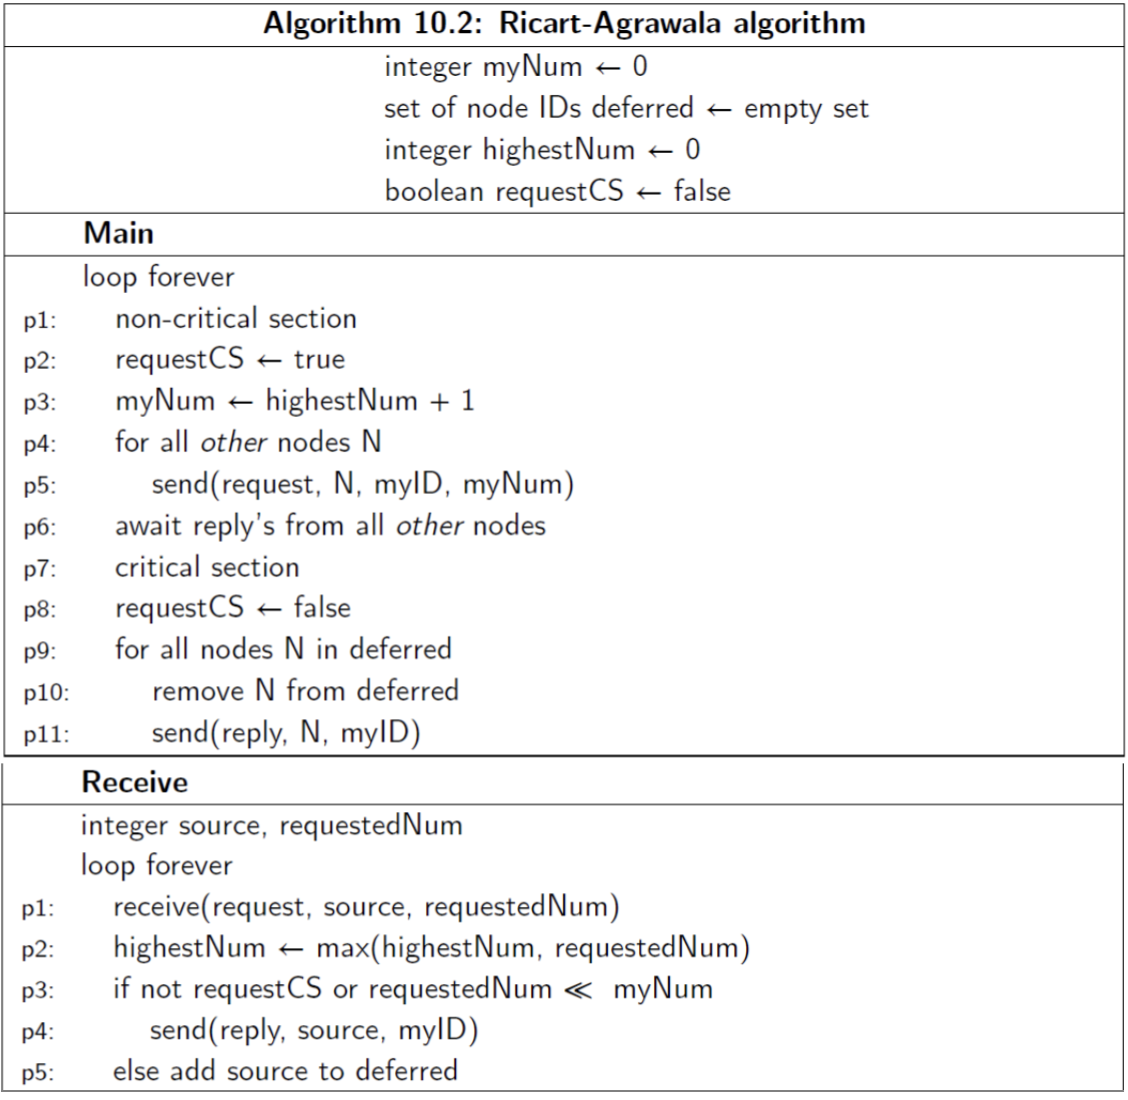
\includegraphics[width=0.9\textwidth]{DV_demand1}
\end{figure}

\begin{Subquestion}
    Suppose that we exchanged the lines $p8$ and $p9-p11$ in Main, i.e. request $CS \leftarrow false$ now executes after the for loop (instead of executing before the for loop). Suppose furthermore that it's possible for \textbf{Receive} to preempt \textbf{Main} at these locations. Provide an example that illustrates why the modified algorithm is no longer correct.
    
\begin{answer}
    Answer:
    \begin{quote}
        Suppose the exchanging $p8$ and $p9-p11$, when a process $p$ is finish and get out from critical section, it send message to all node N in deferred, during this period, the Receive part of $P$ check the requestCS of itself is true, and it will record the source into defer. Suppose the receiver accept the request and put them in defer, the loop may go on forever, and causing that process $P$ may not apply to enter the Critical section again.\\
    \end{quote}
\end{answer}
\end{Subquestion}

\clearpage
\begin{Subquestion}
    In \textbf{Receive}, can the statement\\\\
    \vspace{1ex}
    \textbf{p2: highestNum $\leftarrow$ max(highestNum,\ requestNum)} be replaced by\\
    \vspace{1ex}
    \textbf{p2: highestNum $\leftarrow$ requestNum}? Why? Justify your answer and provide an example.
    
\begin{answer}
    Answer:
    \begin{quote}
        Suppose there is a request message sent to $P$ which be delay by some ways, during this time, more request which have high marks had been accepted by $P$. If the grogram only copy request number as the highestNum, it may choose a less number, and it may appear two or more request message with same requestNum which send by different process, receive part $p3$ find the requestNum is not smaller than my number, and record them, it may lead that some process cannot get reply from all node and cannot go into critical section.\\ 
    \end{quote}
\end{answer}
\end{Subquestion}
\end{Question}


\clearpage
\setcounter{question}{2}

\begin{Question} [\large\textbf {Token-Passing{[4 points]}}]
    Pseudocode of the Ricart-Agrawala Token-passing Algorithm is:
\begin{figure}[H]
    \centering 
    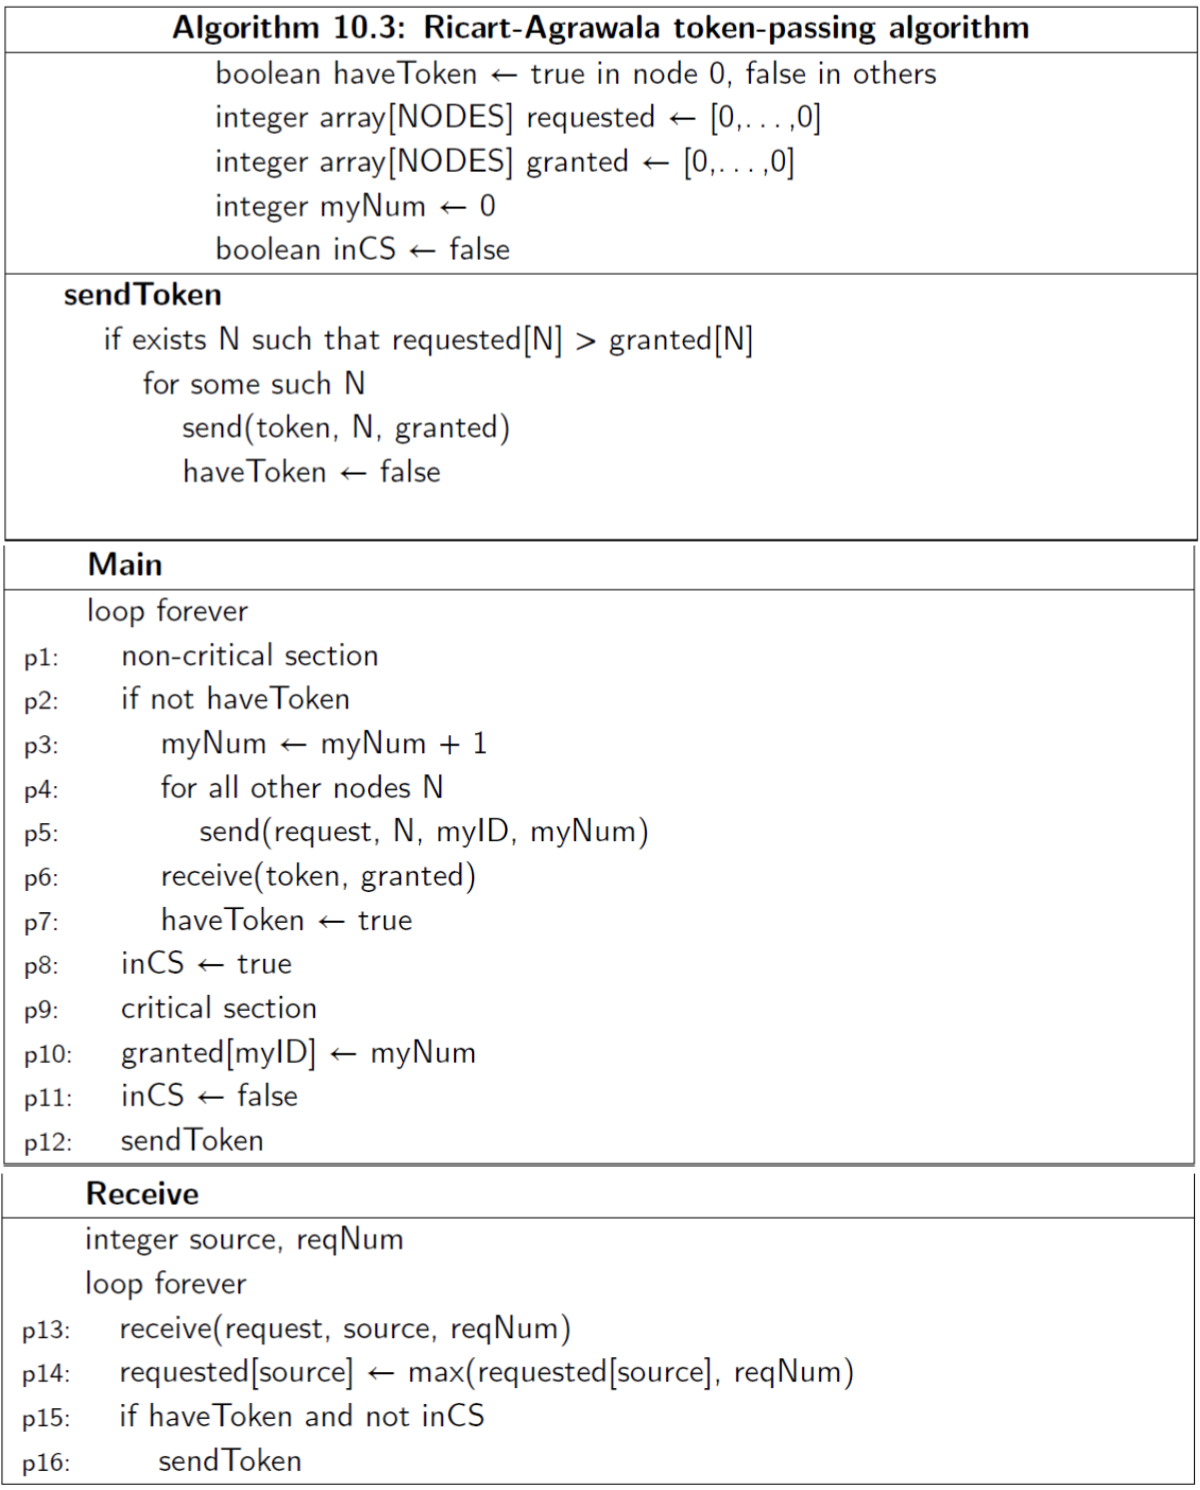
\includegraphics[width=0.9\textwidth]{DV_demand2}
\end{figure}

\clearpage
\begin{Subquestion}
    In node $i$, can the value of \textbf{requested$[j]$} be less than the value of \textbf{granted$[j]$} for $j \neq i$? Why? Justify your answer.
    
\begin{answer}
    Answer:
    \begin{quote}
        Yes. Suppose a process $P$ send a message for all of the node and get the token, one of the other process $Q$ have not get the request message or message had been lost, when this process $Q$ get the token, it will appear that the request times of the $P$ is less than the granted of $P$.\\
    \end{quote}
\end{answer}
\end{Subquestion}

\begin{Subquestion}
    In node $i$, can the value of \textbf{requested$[j]$} be greater than the value of \textbf{granted$[j]$} for $j \neq i$? Why? Justify your answer.
    
\begin{answer}
    Answer:
    \begin{quote}
        Yes. When there are more than one process $p$, $q$... which send request message, the process which had token need to choose one of it, suppose it is $p$ and send the token. During this time, the process $q$ send the second or more request and get by the process $p$ which get the token, the request times of $q$ will larger than the granted time of $p$.\\
    \end{quote}
\end{answer}
\end{Subquestion}
\end{Question}


\end{document}